\documentclass[12pt]{article}
\usepackage[margin=1in]{geometry}
\usepackage{amsthm,amssymb}
\usepackage{amsmath}
\usepackage{amsfonts}
\usepackage{amssymb}
\usepackage{physics}
\newcommand{\N}{\mathbb{N}}
\newcommand{\R}{\mathbb{R}}
\newcommand{\Z}{\mathbb{Z}}
\newcommand{\Q}{\mathbb{Q}}
\newcommand{\matr}[1]{\mathbf{#1}}
\newenvironment{theorem}[2][Theorem]{\begin{trivlist}
\item[\hskip \labelsep {\bfseries #1}\hskip \labelsep {\bfseries #2.}]}{\end{trivlist}}
\newenvironment{lemma}[2][Lemma]{\begin{trivlist}
\item[\hskip \labelsep {\bfseries #1}\hskip \labelsep {\bfseries #2.}]}{\end{trivlist}}
\newenvironment{exercise}[2][Exercise]{\begin{trivlist}
\item[\hskip \labelsep {\bfseries #1}\hskip \labelsep {\bfseries #2.}]}{\end{trivlist}}
\newenvironment{problem}[2][Problem]{\begin{trivlist}
\item[\hskip \labelsep {\bfseries #1}\hskip \labelsep {\bfseries #2.}]}{\end{trivlist}}
\newenvironment{question}[2][Question]{\begin{trivlist}
\item[\hskip \labelsep {\bfseries #1}\hskip \labelsep {\bfseries #2.}]}{\end{trivlist}}
\newenvironment{corollary}[2][Corollary]{\begin{trivlist}
\item[\hskip \labelsep {\bfseries #1}\hskip \labelsep {\bfseries #2.}]}{\end{trivlist}}


\usepackage{xspace}
\newcommand{\A}{\ensuremath{\mathcal{A}}\xspace}
\newcommand{\B}{\ensuremath{\mathcal{B}}\xspace}
\newcommand\pa[1]{\ensuremath{\left(#1\right)}}

%For the infografic
\usepackage{tikz,times}
%\usepackage[paperwidth=25cm,paperheight=22cm,left=1cm,top=1cm]{geometry}
\usetikzlibrary{mindmap,backgrounds}
\usepackage{xcolor}
\usepackage{color}

% Example: download a usepackage 
%\usepackage{CJK}


% For the code
\usepackage{listings}
\usepackage{pythonhighlight}


% for tables
\usepackage{adjustbox}
\usepackage[flushleft]{threeparttable}
%\usepackage[labelfont=sc]{caption}





\begin{document}

\definecolor{bitter}{rgb}{1.0, 0.46, 0.09}
\definecolor{redalt}{rgb}{0.65, 0.0, 0.0}
\definecolor{citrine}{rgb}{0.9, 0.9,0}

\title{Problem Set 5}
\author{Milton Straw\\
ECON 815: Topics in Microeconomics}
\date{Fall 2019}
\maketitle

\textsc{Description.}\\

My interest in health economics had me thinking about survival analysis. Since it's not something we've done in class before, it was an opportunity for me to dig on the Internet, find the correct packages necessary, and learn some of the basics of implementing survival analysis in Python. I've done some exercises in Stata before, so I did the Stata-work initially to guide what I wanted to do in Python. \\

The data used is just an example set for the purpose of this exercise. It isn't a real dataset.\\

\textsc{Visualizations.}

\begin{figure}[!h]
	\centering
	\centering
	\caption{Kaplan Meier Survivor Function}
	\label{fig:kaplanmeier}
	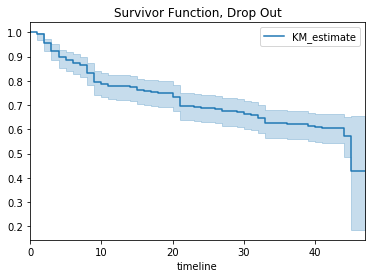
\includegraphics[scale=0.5]{fig1.png}
\end{figure}

\begin{figure}[!h]
	\centering
	\centering
	\caption{Nelson Aalen Cumulative Hazard Function}
	\label{fig:nelsonaalen}
	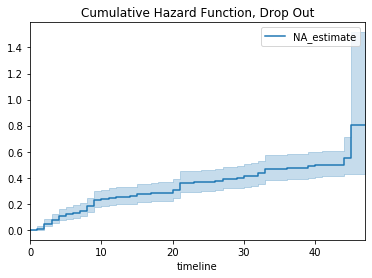
\includegraphics[scale=0.5]{fig2.png}
\end{figure}

\begin{figure}[!h]
	\centering
	\centering
	\caption{Cox Proportional Hazard Model}
	\label{fig:cox}
	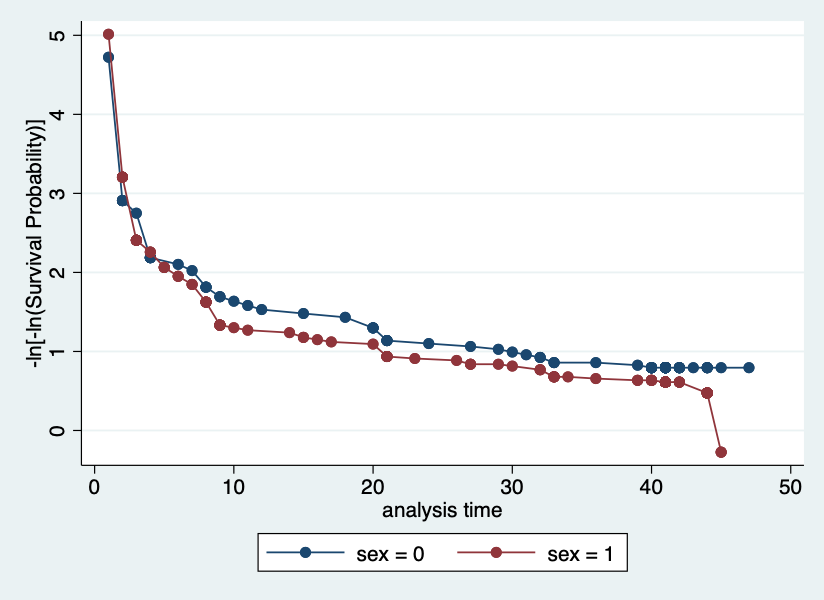
\includegraphics[scale=0.5]{cph.png}
\end{figure}



\end{document}